% begin module polar-intro
\begin{frame}
\frametitle{(11.3)  Polar Coordinates}
\begin{itemize}
\item  The polar coordinates system is an alternative to the Cartesian coordinates system.
%\item  Instead of specifying horizontal distance and vertical distance, we specify angle and distance from the origin.
\item  Choose a point in the plane called $O$ (the origin).
\item  Draw a ray starting at $O$ called the polar axis.  This ray is usually drawn horizontally to the right.
\end{itemize}
\begin{columns}[c]
\column{.5\textwidth}
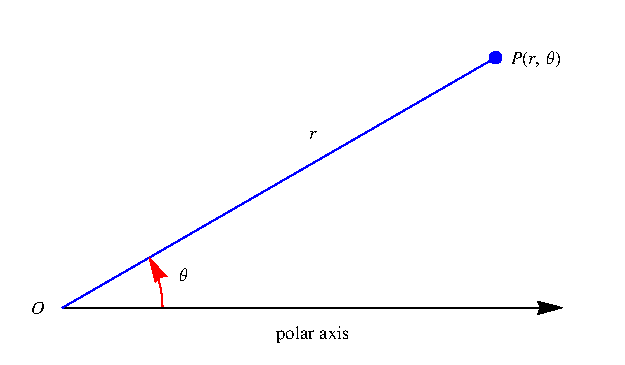
\includegraphics[height=4cm]{polar-curves/pictures/11-03-polar.pdf}%
\column{.5\textwidth}
\begin{itemize}
\item  Let $P$ be a point in the plane.
\item  Let $\theta$ denote the angle between the polar axis and the line $OP$.
\item  Let $r$ denote the length of the line $OP$.
\item  Then $P$ is represented by the ordered pair $(r, \theta )$.
\end{itemize}
\end{columns}
\end{frame}
% end module polar-intro
